\documentclass[14pt,a4paper,report]{report}
\usepackage[a4paper, mag=1000, left=2.5cm, right=1cm, top=2cm, bottom=2cm, headsep=0.7cm, footskip=1cm]{geometry}
\usepackage[utf8]{inputenc}
\usepackage[english,russian]{babel}
\usepackage{indentfirst}
\usepackage[dvipsnames]{xcolor}
\usepackage[colorlinks]{hyperref}
\usepackage{listings} 
\usepackage{fancyhdr}
\usepackage{caption}
\usepackage{amsmath}
\usepackage{latexsym}
\usepackage{graphicx}
\usepackage{amsmath}
\usepackage{booktabs}
\usepackage{array}
\hypersetup{
 colorlinks = true,
 linkcolor  = black
}

\usepackage{listings}
\usepackage{caption}
\DeclareCaptionFont{white}{\color{white}}
\DeclareCaptionFormat{listing}{\colorbox{gray}{\parbox{\dimexpr\textwidth-1.72\fboxsep\relax}{#1#2#3}}}
\captionsetup[lstlisting]{format=listing,labelfont=white,textfont=white,margin=0pt}
\lstset{language=C,
	basicstyle=\footnotesize,
	keepspaces=true,
	tabsize=4,               
	frame=single,                           % Single frame around code
	rulecolor=\color{black},
	captionpos=b,
	showstringspaces=false,	
	abovecaptionskip=-0.9pt,
	xleftmargin=3.4pt,
	xrightmargin=2.6pt,
	breaklines=true,
	postbreak=\raisebox{0ex}[0ex][0ex]{\ensuremath{\color{black}\hookrightarrow\space}},
	xleftmargin=3.2pt,
	literate={а}{{\selectfont\char224}}1
	{~}{{\textasciitilde}}1
	{б}{{\selectfont\char225}}1
	{в}{{\selectfont\char226}}1
	{г}{{\selectfont\char227}}1
	{д}{{\selectfont\char228}}1
	{е}{{\selectfont\char229}}1
	{ё}{{\"e}}1
	{ж}{{\selectfont\char230}}1
	{з}{{\selectfont\char231}}1
	{и}{{\selectfont\char232}}1
	{й}{{\selectfont\char233}}1
	{к}{{\selectfont\char234}}1
	{л}{{\selectfont\char235}}1
	{м}{{\selectfont\char236}}1
	{н}{{\selectfont\char237}}1
	{о}{{\selectfont\char238}}1
	{п}{{\selectfont\char239}}1
	{р}{{\selectfont\char240}}1
	{с}{{\selectfont\char241}}1
	{т}{{\selectfont\char242}}1
	{у}{{\selectfont\char243}}1
	{ф}{{\selectfont\char244}}1
	{х}{{\selectfont\char245}}1
	{ц}{{\selectfont\char246}}1
	{ч}{{\selectfont\char247}}1
	{ш}{{\selectfont\char248}}1
	{щ}{{\selectfont\char249}}1
	{ъ}{{\selectfont\char250}}1
	{ы}{{\selectfont\char251}}1
	{ь}{{\selectfont\char252}}1
	{э}{{\selectfont\char253}}1
	{ю}{{\selectfont\char254}}1
	{я}{{\selectfont\char255}}1
	{А}{{\selectfont\char192}}1
	{Б}{{\selectfont\char193}}1
	{В}{{\selectfont\char194}}1
	{Г}{{\selectfont\char195}}1
	{Д}{{\selectfont\char196}}1
	{Е}{{\selectfont\char197}}1
	{Ё}{{\"E}}1
	{Ж}{{\selectfont\char198}}1
	{З}{{\selectfont\char199}}1
	{И}{{\selectfont\char200}}1
	{Й}{{\selectfont\char201}}1
	{К}{{\selectfont\char202}}1
	{Л}{{\selectfont\char203}}1
	{М}{{\selectfont\char204}}1
	{Н}{{\selectfont\char205}}1
	{О}{{\selectfont\char206}}1
	{П}{{\selectfont\char207}}1
	{Р}{{\selectfont\char208}}1
	{С}{{\selectfont\char209}}1
	{Т}{{\selectfont\char210}}1
	{У}{{\selectfont\char211}}1
	{Ф}{{\selectfont\char212}}1
	{Х}{{\selectfont\char213}}1
	{Ц}{{\selectfont\char214}}1
	{Ч}{{\selectfont\char215}}1
	{Ш}{{\selectfont\char216}}1
	{Щ}{{\selectfont\char217}}1
	{Ъ}{{\selectfont\char218}}1
	{Ы}{{\selectfont\char219}}1
	{Ь}{{\selectfont\char220}}1
	{Э}{{\selectfont\char221}}1
	{Ю}{{\selectfont\char222}}1
	{Я}{{\selectfont\char223}}1,
	extendedchars=true
}

\definecolor{MyDarkGreen}{rgb}{0.0,0.4,0.0}

\usepackage{titlesec}
\titleformat{\chapter}
{\Large\bfseries} % format
{}                % label
{0pt}             % sep
{\huge}           % before-code


\DeclareCaptionFont{white}{\color{white}} 

% Listing description
\usepackage{listings} 
\DeclareCaptionFormat{listing}{\colorbox{gray}{\parbox{\textwidth}{#1#2#3}}}
\captionsetup[lstlisting]{format=listing,labelfont=white,textfont=white}
\lstloadlanguages{Matlab}%
\lstset{language=Matlab,                        % Use MATLAB
        frame=single,                           % Single frame around code
        basicstyle=\small\ttfamily,             % Use small true type font
        keywordstyle=[1]\color{Blue}\bfseries,        % MATLAB functions bold and blue
        keywordstyle=[2]\color{Purple},         % MATLAB function arguments purple
        keywordstyle=[3]\color{Blue}\underbar,  % User functions underlined and blue
        identifierstyle=,                       % Nothing special about identifiers
                                                % Comments small dark green courier
        commentstyle=\usefont{T1}{pcr}{m}{sl}\color{MyDarkGreen}\small,
        stringstyle=\color{Purple},             % Strings are purple
        showstringspaces=false,                 % Don't put marks in string spaces
        tabsize=5,                              % 5 spaces per tab
        %
        %%% Put standard MATLAB functions not included in the default
        %%% language here
        morekeywords={xlim,ylim,var,alpha,factorial,poissrnd,normpdf,normcdf},
        %
        %%% Put MATLAB function parameters here
        morekeywords=[2]{on, off, interp},
        %
        %%% Put user defined functions here
        morekeywords=[3]{FindESS, homework_example},
        %
        morecomment=[l][\color{Blue}]{...},     % Line continuation (...) like blue comment
        numbers=left,                           % Line numbers on left
        firstnumber=1,                          % Line numbers start with line 1
        numberstyle=\tiny\color{Blue},          % Line numbers are blue
        stepnumber=5                            % Line numbers go in steps of 5
        }


\begin{document}

\def\contentsname{Содержание}

% Titlepage
\begin{titlepage}
 \begin{center}
  \textsc{Санкт-Петербургский Политехнический 
   Университет Петра Великого\\[5mm]
   Кафедра компьютерных систем и программных технологий}
  
  \vfill
  
  \textbf{Отчёт по лабораторной работе №1\\[3mm]
   Курс: «Методы оптимизации и принятия решений»\\[3mm]
   Тема: «Многокритериальная оптимизация»\\[35mm]
   }
 \end{center}
 
 \hfill
 \begin{minipage}{.5\textwidth}
  Выполнил студент:\\[2mm] 
Ерниязов Тимур Ертлеуевич\\
  Группа: 13541/2\\[5mm]
  
  Проверил:\\[2mm] 
  Сиднев Александр Георгиевич
 \end{minipage}
 \vfill
 \begin{center}
  Санкт-Петербург\\ \the\year\ г.
 \end{center}
\end{titlepage}

% Contents
\tableofcontents
\clearpage

\chapter{Лабораторная работа №1}

\section{Цель работы}

Научиться решать задачи по многокритериальной оптимизации.

\section{Программа работы}

\begin{enumerate}
    \item Осуществить переход от многокритериальной задачи к однокритериальной с использованием следующих подходов:
    
\begin{itemize}
 \item Выделение главного критерия
 \item Свертка критериев (аддитивная и мультипликативная)
 \item Максимин или минимакс (он же метод максиминной свертки)
 \item Метод последовательных уступок
 \item fgoalattain
 \item Ведение метрики в пространстве критериев
\end{itemize}

    \item  Решить задачу стохастического программирования для одной из однокритериальных задач, превратив детерминированное ограничение в вероятностное по схеме
   
   $$ P(\sum_{j=1}^n a_{ij}x_{ij} - b_{ij} \leq 0) \geq a_i$$
   
Менять  $ a_i $  в следующем диапазоне $ 0.1 \leq a_i \leq 0.9 $.

Считать случайной величиной $b_i$  или элементы   $ {a_{ij}}i$-й строки матрицы  А  (по выбору).

Разрешается изменить формулировку исходной задачи, придумать собственную задачу, найти другую аналогичную задачу, которая могла бы быть сформулирована как многокритериальная.
\end{enumerate}

\section{Индивидуальное задание}

\subsubsection{Задача 7}

Студент 5 курса Олег 28го декабря возвращается из предновогодней поездки к родственникам в братское государство Украина с важным заданием от студентов своего потока: закупить провизии для совместного празднования всем потоком Нового Года.

В ходе жарких споров и голосований был составлен список провианта, который должен купить Олег. Так как Олег, подобно большинству студентов, ленив и делает все в последний момент, он закупается в день уезда в продуктовом магазине неподалеку от бабушкиной квартиры. Естественно, в магазине ему удалось найти не все продукты из списка.

Вот провиант, который можно купить:

\begin{table}[]
\resizebox{\textwidth}{!}{%
\begin{tabular}{|l|l|l|l|l|l|}
\hline
Провиант & Эффект & Последствия & Вкус & Масса & Цена \\ \hline
Шампанское & 0.5 & 0.9 & 0.3 & 0.3 & 50 \\ \hline
Водка & 2 & 8 & 0 & 1 & 30 \\ \hline
Свежавыжитый сок & 0 & 0 & 5 & 1 & 30 \\ \hline
Коктейли & 0 & 0 & 4 & 1 & 50 \\ \hline
Коньяк & 5 & 2 & 1 & 1 & 70 \\ \hline
Салаты & 0 & 0 & 5 & 0.5 & 20 \\ \hline
\end{tabular}%
}
\end{table}

Студенческий совет выработал следующие правила покупки провианта:

\begin{itemize}
    \item Эффект, прибавленный к вкусу, должен быть максимизирован.
    \item Последствия следует минимизировать.
    \item Необходимо купить не более 3 литров водки и не более 5 литров коньяка (т.к. Олег учится на ФЭМе и у него очень мало парней в группе).
\end{itemize}

Помимо этого, девушки в совете выдвинули следующее условие:

\begin{itemize}
    \item Необходимо купить как минимум 3 литра свежевыжатого сока и 2 литра вкусных безалкогольных коктейлей (да-да, это же девушки).
\end{itemize}
Естественно, необходимо потратить как можно меньше денег (гривен).

Следующая проблема заключается в том, что Олег везет весь провиант через границу. 25 литров Олег готов распихать по соседям, но если придется везти большее количество провианта, Олегу придется дать взятку украинским пограничникам в размере 100 гривен за каждый лишний литр. Если Олег возьмет с собой больше 100 литров, его арестуют как контрабандиста.





\subsection{Математическая модель задачи многокритериальной оптимизации}

Введем обозначения:
\begin{itemize}
    \item $x_1$ - количество шампанского 
    \item $x_2$ - количество водки
    \item $x_3$ - количество сока
    \item $x_4$ - количество коктейлей
    \item $x_5$ - количество коньяка
    \item $x_6$ - количество салатов
\end{itemize}

\subsubsection{Критерии:}

\begin{enumerate}
\item Эффект плюс вкус должен быть максимизирован $$ f_1 = 0.8x_1+2x_2+5x_3+4x_4+6x_5_+5x_6 -> max$$
\item Последствия минимизированы $$ f_2 = 0.9x_1+8x_2+2x_5 -> min$$
\item Необходимо потратить как можно меньше денег
\begin{enumerate}Вес провианта меньше  25 $$ f_3 = 50x_1+30x_2+30x_2+50x_4+70x_5+20x_6 -> min$$
\item Вес провианта больше или равен 25 (Взятка 100 гривен за каждый превышенный литр) $$ f_3 = 50x_1+30x_2+30x_2+50x_4+70x_5+20x_6 + 100(0.3x_1+x_2+x_3+x_4+x_5+0.5x_6-25) ->min$$
\end{enumerate}
\end{enumerate}

\subsubsection{Ограничения:}

\begin{enumerate}
    \item по общему весу провианта $$ 0.3x_1+x_2+x_3+x_4+x_5+0.5x_6 < 100 $$
    \item по весу каждого провианта 
    $$ 0 \leq x_1 \leq 100   $$
        $$ 0 \leq x_2 \leq 3   $$
    $$ 3 \leq x_3 \leq 100   $$
    $$ 2 \leq x_4 \leq 100   $$
    $$ 0 \leq x_5 \leq 5   $$
    $$ 0 \leq x_6 \leq 100   $$
    
\end{enumerate}


Запишем все в систему уравнений:

\begin{equation*}
 \begin{cases}
     0.3x_1+x_2+x_3+x_4+x_5+0.5x_6 < 100  \\
     0 \leq x_1 \leq 100  \\
     0 \leq x_2 \leq 3   \\
     3 \leq x_3 \leq 100   \\
     2 \leq x_4 \leq 100   \\
     0 \leq x_5 \leq 5  \\
     0 \leq x_6 \leq 100   \\
 \end{cases}
\end{equation*}


 



\subsection{Поиск оптимумов частных критериев}
Найдем оптимумы каждой из целевых функций независимо от других. Для этого необходимо решить три задачи однокритериальной оптимизации.

\begin{enumerate}

     \item $$ f_1 = 0.8x_1+2x_2+5x_3+4x_4+6x_5_+5x_6 -> max$$
 при

\begin{equation*}
 \begin{cases}
     0.3x_1+x_2+x_3+x_4+x_5+0.5x_6 < 100  \\
     0 \leq x_1 \leq 100  \\
     0 \leq x_2 \leq 3   \\
     3 \leq x_3 \leq 100   \\
     2 \leq x_4 \leq 100   \\
     0 \leq x_5 \leq 5  \\
     0 \leq x_6 \leq 100   \\
 \end{cases}
\end{equation*}

     \item $$ f_2 = 0.9x_1+8x_2+2x_5 -> min$$
при

\begin{equation*}
 \begin{cases}
     0.3x_1+x_2+x_3+x_4+x_5+0.5x_6 < 100  \\
     0 \leq x_1 \leq 100  \\
     0 \leq x_2 \leq 3   \\
     3 \leq x_3 \leq 100   \\
     2 \leq x_4 \leq 100   \\
     0 \leq x_5 \leq 5  \\
     0 \leq x_6 \leq 100   \\
 \end{cases}
\end{equation*}

     \item  $$ f_3 = 50x_1+30x_2+30x_2+50x_4+70x_5+20x_6 -> min $$ , при $$0.3x_1+x_2+x_3+x_4+x_5+0.5x_6<25$$
 $$f_3 = 50x_1+30x_2+30x_2+50x_4+70x_5+20x_6 + 100(0.3x_1+x_2+x_3+x_4+x_5+0.5x_6-25)->min $$, при $$0.3x_1+x_2+x_3+x_4+x_5+0.5x_6>=25$$
 
, при

\begin{equation*}
 \begin{cases}
     0.3x_1+x_2+x_3+x_4+x_5+0.5x_6 < 100  \\
     0 \leq x_1 \leq 100  \\
     0 \leq x_2 \leq 3   \\
     3 \leq x_3 \leq 100   \\
     2 \leq x_4 \leq 100   \\
     0 \leq x_5 \leq 5  \\
     0 \leq x_6 \leq 100   \\
 \end{cases}
\end{equation*}
\end{enumerate}
Для решение данной задачи, был использован MATLAB.

\lstinputlisting{listings/0.m}

Получили следующие значения:
\lstinputlisting{listings/1.m}

Как видно, три отдельных критерия работают плохо, так как задача минимизировать расход приводит к тому, что можно ничего не покупать (кроме минимума для девочек).









\section{Переход от многокритериальной задачи к однокритериальной}
\subsection{Выделение главного критерия}


Один из критериев - главный - имеет существенно более высокий приоритет, чем все остальные, но по остальным критериям вариант тоже не должен быть слишком плох. Пусть главный критерий - первый, следовательно, для оставшихся целевых функций необходимо указать нижние границы. Для того, чтобы функция включала в себя провиант с последствиями, сделаем ограничения в последствиях чуть больше 30. Установим бюдет равный 5000 гривн.


$$ f_1 = 0.8x_1+2x_2+5x_3+4x_4+6x_5_+5x_6 -> max$$
 при

\begin{equation*}
 \begin{cases}
    0.9x_1+8x_2+2x_5 > 50\\
     f = 0.3x_1+x_2+x_3+x_4+x_5+0.5x_6  \\
     f<100 \\
     0 \leq x_1 \leq 100  \\
     0 \leq x_2 \leq 3   \\
     3 \leq x_3 \leq 100   \\
     2 \leq x_4 \leq 100   \\
     0 \leq x_5 \leq 5  \\
     0 \leq x_6 \leq 100   \\
     50x_1+30x_2+30x_2+50x_4+70x_5+20x_6 + 100(f-25) < 5000  & f>=25 \\
          50x_1+30x_2+30x_2+50x_4+70x_5+20x_6 < 5000  & f<25 \\
     
 \end{cases}
\end{equation*}


В соответствии с изменениями скрипт был дополнен ограничениями.
\lstinputlisting{listings/3.m}

После выполнения программы были получены следующие результаты:
\lstinputlisting{listings/4.m}

Все ограничения учтены.



















\subsection{Свертка критериев}
\subsubsection{Аддитивная свертка критериев}
Для использования метода аддитивной свертки необходимо выполнить нормировку критериев, с тем чтобы сделать их значения соизмеримыми, а единицы измерения – безразмерными. Выполним нормировку следующим образом:
    
    
\begin{equation}
\overline{z_1} = \frac{z_1}{|z_1^{min}|} = - \frac{0.8x_1+2x_2+5x_3+3x_4+6x_5+5x_6}{753} 
\end{equation}

\begin{equation}
\overline{f_2} = \frac{f_2}{|f_2^{min}|}= \frac{0.9x_1+8x_2+2x_5}{0.1}
\end{equation}

\begin{equation}
\overline{f_3} = \frac{f_3}{|f_3^{min}|} = \frac{50x_1+30x_2+30x_3+50x_4+70x_5+20x_6}{190} 
\end{equation}
, при  $$0.3x_1+0.5x_6+x_2+x_3+x_4+x_5<25$$
\begin{equation}
\overline{f_3} = \frac{f_3}{|f_3^{min}|} = \frac{50x_1+30x_2+30x_3+50x_4+70x_5+20x_6+100(0.3x_1+0.5x_6+x_2+x_3+x_4+x_5-25)}{190} 
\end{equation}
, при $$0.3x_1+0.5x_6+x_2+x_3+x_4+x_5>=25$$

Формула аддитивной свертки имеет вид:
\begin{equation}
F(x) = \sum_{i=1}^{r}\lambda_i f_i(x), 0<\lambda_i<1, \sum_i^{}\lambda_i=1,
\end{equation}
где $f_i(x)$ - критерии оптимальности, $r$ – их общее число, а $\lambda_i$ - параметры важности. 

\lstinputlisting{listings/5.m}

После выполнения программы были получены следующие результаты:
\lstinputlisting{listings/6.m}


Результат:
\begin{itemize}
\item 38 - показатель эффекта + вкуса
\item 0,0528 - показатель последствий
\item 297.88 гривны - стоимость покупки
\end{itemize}

Метод не плох, но опять минимизация стоимости покупки хоть и с коэффициентом 0.2 очень сильно влияет на оптимизацию и в результате получаеться, что лучше вообще ничего не покупать.

























\subsubsection{Мультипликативная свертка критериев}
Формула мультипликативной свертки имеет вид:
\begin{equation}
F(x) = \prod_{i=1}^{r}f_i(x)^{\lambda_i}
\end{equation}
где $f_i(x)$ - критерии оптимальности, $r$ - их общее число, а $\lambda_i$ - показатели важности. Нормировка уже была произведена в аддитивной свертки, в итоге получим следующую задачу однокритериальной оптимизации.




\lstinputlisting{listings/7.m}

После выполнения программы были получены следующие результаты:

\lstinputlisting{listings/8.m}

Результат:
\begin{itemize}
\item 38.185 - показатель эффекта + вкуса
\item 0.052818 - последствия
\item 299.58 гривн - стоимость 
\end{itemize}

Свертка привела к неплохим результатам. 


























\subsection{Минимакс (максимин)}
Максиминную свертку представим в следующем виде: $C_i(a)= \text{min } w_i C_i(a)$

Решение $a^*$ является наилучшим, если для всех $a$ выполняется условие $C(a^*) \geq C(a)$, или $a^* = \text{arg max } C(a) = \text{arg max min } w_i C_i (a)$.

Для реализации максиминной свертки необходимо в fminimax передавать функции обратные целевым (функция funminmax). Так как оцениваемые показатели разновелики, необходимо нормировать критерии. Что было произведено ранее.

\lstinputlisting{listings/10.m}
После выполнения программы были получены следующие результаты:
\lstinputlisting{listings/9.m}

Результат:
\begin{itemize}
\item 38.495 - показатель Э+В
\item 7.6421 - показатель последствий
\item 361.58 гривн - стоимость 
\end{itemize}































\subsection{Метод последовательных уступок}
Для решения данной задачи была выбрана уступка = 10\%. 	Предположим, что критерии пронумерованы в следующем порядке важности:
\begin{center}
$f_1>f_3>f_2$
\end{center} 

Для первого критерия уже решена задача поиска оптимального значения в п 1.2.1. То есть:
\begin{center}
$753 * 0.9 = 677.7$
\end{center}


\lstinputlisting{listings/11.m}
После выполнения программы были получены следующие результаты:
\lstinputlisting{listings/12.m}

В соответствии с полученным значением введем ограничение для второго критерия.

\begin{center}
$ 9212.2 * 0.9 = 8290.98 $
\end{center}

Ограничения критерия выглядит следующим образом:

\lstinputlisting{listings/14.m}

После выполнения программы были получены следующие результаты:
\lstinputlisting{listings/13.m}


Результат:
\begin{itemize}
\item 399.84 - показетль Э+В
\item 124 - показатель последствий
\item 13322 гривны - стоимость
\end{itemize}






























\subsection{Метод достижения цели (fgoalattain)}
Fgoalattain решает задачу достижения цели, которая является одной из формулировок задач для векторной оптимизации.
x = fgoalattain(fun, $x_0$, goal, weight, ...):
\begin{itemize}
\item fun – целевая функция,
\item $x_0$ – начальные значения,
\item goal – целевые значения,
\item weight – веса.
\end{itemize}
Пусть goal = ($z_1^{min}, f_2^{min}, z_3^{min}$), w = ($|z_1^{min}|, |f_2^{min}|, |z_3^{min}|$). Тогда скрипт для решения задачи будет выглядеть следующим образом:

\lstinputlisting{listings/16.m}
После выполнения программы были получены следующие результаты:
\lstinputlisting{listings/15.m}


Результат:
\begin{itemize}
\item 49 - показатель Э+В
\item 0.0000000019 - показатель последствий
\item 367 гривны - стоимость
\end{itemize}

Результаты fgoalattain на 93 процента хуже цели.



















\subsection{Введение метрики в пространстве критериев}

Для перехода к однокритериальной задаче оптимизации методом введения метрики в пространстве целевых функций необходимо определить координаты «идеальной» точки $a=(f_1^*, f_2^*, ..., f_r^*)$,  где $f_i = min f_i(x)$. Эти значения
уже были получены в п. 1.2.1, и поэтому:




Введем в пространстве критериев метрику в виде евклидова расстояния:
\begin{equation}
p(y, a) = [\sum_{i=1}^r(a_i-y_i)^2]^{\frac{1}{2}} 
\end{equation}
Тогда за целевую функцию (обобщенный критерий), с учётом необходимости нормировки, можно взять выражение:
\begin{equation}
f=\sum_{i=1}^r(\frac{a_i-f_i}{f_i^*})^2=\sum_{i=1}^r(1-\frac{f_i}{f_i^*})^2
\end{equation}
Таким образом, получаем следующую задачу оптимизации:
\begin{equation}
f=(1-\frac{z_1}{z_1^{min}})^2+(1-\frac{z_2}{z_2^{min}})^2+(1-\frac{f_3}{f_3^{min}})^2
\end{equation}

\lstinputlisting{listings/18.m}
После выполнения программы были получены следующие результаты:
\lstinputlisting{listings/17.m}

Результат:
\begin{itemize}
\item 37.045 - показатель Э+В
\item 0.05525 - показатель последствий
\item 291.63 гривны - стоимость
\end{itemize}


















\clearpage


\section{Оценка Парето-оптимальности полученных решений}
Для того чтобы уменьшить количество альтернатив, среди которых лицо, принимающее решение (ЛПР), должно сделать выбор, можно выделить множество Парето среди всех полученных решений. Для этого была составлена таблица и построен график.

\begin{table}[h!]
\begin{tabular}{|l|l|l|l|l|}
\hline
Метод & f_1 & f_2 & f_3\\ \hline
Выделение главного критерия                 & 369.4921 & 50 & 5000     \\ \hline
 Аддитивная свертка                         & 38 & 0.0528 & 297.88     \\ \hline
 Мультипликативная свертка                  & 38.185 & 0.052818 & 299.58     \\ \hline
Минимакс                                    & 38.495 & 7.6421 & 361.58     \\ \hline
Метод последовательных уступок              & 399.84 & 124 & 13322     \\ \hline
fgoalattain                                 & 49 & 0 & 367    \\ \hline
 Введение метрики в пространстве критериев  & 37.045 & 0.055 & 291.63     \\ \hline

\end{tabular}
\end{table}

\begin{figure}[h!]
	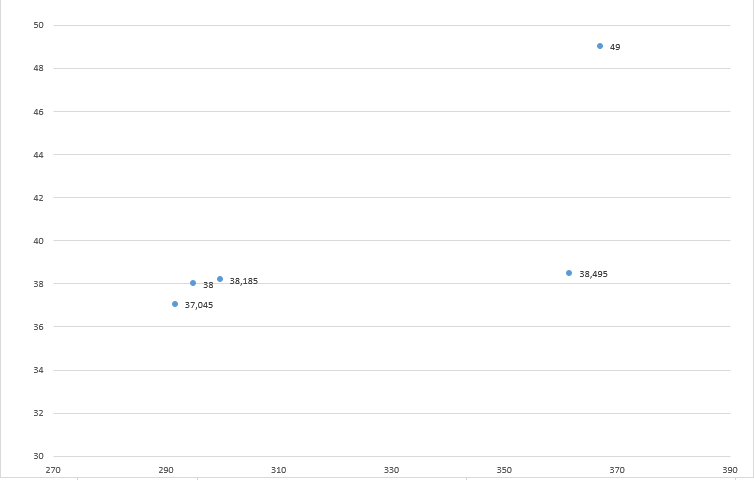
\includegraphics[width=\textwidth]{img/1.png}
	\caption{Оценки от полученных решений на плоскости критериев}
\end{figure}  


Паррето-оптимальным являеться точка 49;367 (fgoalattain показал лучшее решение). В графике не были учетны точки выделения главного критерия и метода последовательных уступков.


























\section{Решение задачи стохастического программирования}
Рассмотрим задачу стохастического программирования на основе задачи однокритериальной оптимизации, которая была получена из исходной методом введения метрики в пространстве критериев.

P-постановка:
$$  W =P(\sum_{j=1}^{n} c_j x_j >=W_{max})->max $$
, где$ W_{max}$ - предварительно заданное допустимое наихудшее (максимальное) значение целевой функции.

Суть P-постановки заключается в том, что необходимо найти такие значения $x_j$, при которых максимизируется вероятность того, что целевая функция будет не хуже предельно допустимого значения.

Ограничения задачи, которые должны выполняться при всех реализациях параметров условий задачи, называются жесткими ограничениями. 

Преобразуем ограничение системы:
\begin{center}
$$ 0.3x_1+x_2+x_3+x_4+x_5+0.5x_6 < 100 $$
\end{center}

и вероятностное тогда:
$$ P(a_1x_1+a_2x_2+a_3x_3+a_4x_4+a_5x_5+a_6x_6 < 100)>=a $$

Вероятностное ограничениестановиться эквивалентно детерминированному неравенству:

$$ 0.3x_1+x_2+x_3+x_4+x_5+0.5x_6+ K_\alpha * \sqrt{x_1^2+x_2^2+x_3^2+x_4^2+x_5^2+x_6^2}$$

\begin{center}
$M(\alpha_{1})=0.3, M(\alpha_{2})=1, M(\alpha_{3})=1, M(\alpha_{4})=1, M(\alpha_{5})=1, M(\alpha_{6})=0.5$
$D(\alpha_{1})=0.15, D(\alpha_{2})=0.5, D(\alpha_{3})=0.5, D(\alpha_{4})=0.5, D(\alpha_{5})=0.5, D(\alpha_{6})=0.25$
\end{center}



Решение задачи представлено как скрипт в программе Matlab

\lstinputlisting{listings/20.m}

Результаты выполнения программы приведены в таблице:

\begin{table}[h!]
\begin{tabular}{|l|l|l|l|l|l|l|l|l|l|}
\hline
a & x_1 & x_2 & x_3 & x_4 & x_5&x_6& f_1 & f_2 & f_3 \\ \hline
0.1& 0.0182& 0.0002& 3.9938& 2.9938& 0.0187& 0.9941& 37.0420& 0.0553& 291.6089 \\ \hline 
0.2& 0.0182& 0.0002& 3.9938& 2.9938& 0.0187& 0.9941& 37.0415& 0.0553& 291.6050 \\ \hline 
0.3& 0.0182& 0.0002& 3.9937& 2.9938& 0.0187& 0.9941& 37.0411& 0.0553& 291.6023 \\ \hline 
0.4& 0.0182& 0.0002& 3.9937& 2.9937& 0.0187& 0.9941& 37.0408& 0.0553& 291.6001 \\ \hline 
0.5& 0.0182& 0.0002& 3.9937& 2.9937& 0.0187& 0.9940& 37.0405& 0.0553& 291.5980 \\ \hline 
0.6& 0.0182& 0.0002& 3.9937& 2.9937& 0.0187& 0.9940& 37.0402& 0.0553& 291.5959 \\ \hline 
0.7& 0.0182& 0.0002& 3.9936& 2.9937& 0.0187& 0.9940& 37.0399& 0.0553& 291.5937 \\ \hline 
0.8& 0.0182& 0.0002& 3.9936& 2.9936& 0.0187& 0.9940& 37.0396& 0.0553& 291.5913 \\ \hline 
0.9& 0.0091& 0.0001& 3.9953& 2.9954& 0.0093& 0.9958& 37.0006& 0.0276& 290.6555 \\ \hline 
\end{tabular}
\end{table}



Для детерминированных ограничений:
X_1 = 0.0182, X_2 = 0.0002, x_3= 3.9937, x_4 =  2.994,x_5 =  0.019,x_6 =  0.994, f1 = 37.04, f2 = 0, f3 = 291.60


Этот метод малочувствителен к параметрам. Значения в таблице практически не меняются.

\end{document}